\documentclass[11pt,letterpaper]{article}

\input{../../../../.config/latex/preamble_v1.tex}
\lightmode

% Disable algorithm numbering
\renewcommand{\thealgocf}{}

\begin{document}

\section*{CS 124 Homework 3: Spring 2022}

\textbf{Your name:} Lev Kruglyak

\textbf{Collaborators:} Swati Goel, Adam Mohamed

\textbf{No. of late days used on previous psets: 4}\\
\textbf{No. of late days used after including this pset: 6}

Homework is due Wednesday at midnight ET. You are allowed up to {\bf twelve} (college)/{\bf forty} (extension school) late days through the semester, but the number of late days you take on each assignme\
nt must be a nonnegative integer at most {\bf two} (college)/{\bf four} (extension school).

Try to make your answers as clear and concise as possible;
style may count in your grades. Assignments must be submitted in pdf format on Gradescope. If you do assignments by hand, you will need to scan in your results to turn them in.

You can collaborate with other students that are currently enrolled in this
course in brainstorming and thinking through approaches to solutions but you should write
the solutions on your own: you must wait one hour after any collaboration or use of notes
from collaboration before any writing in your own solutions that you will submit. 

For all homework problems where you are asked to give an algorithm, you must prove the correctness
of your algorithm and establish the best upper bound that you can give for the running time. Generally
better running times will get better credit; generally exponential time algorithms (unless specifically asked
for) will receive no or little credit. You should always write a clear informal description of your algorithm
in English. You may also write pseudocode if you feel your informal explanation requires more precision
and detail, but keep in mind pseudocode does NOT substitute for an explanation. Answers that consist
solely of pseudocode will receive little or not credit. Again, try to make your answers clear and concise.

\pagebreak
\begin{problem}
    Explain how to solve the following two problems using heaps.  (No credit if you're not using heaps!)  
    \begin{enumerate}[(a)]
        \item {\bf (12 points)} Give an $O(n \log k)$ algorithm to merge $k$ sorted lists with $n$ total elements into one sorted list.
        \item {\bf (12 points)} Say that a list of numbers is $k$-close to sorted if each number in the list is less than $k$ positions from its actual place in the sorted order.  (Hence, a list that is 1-close to sorted is actually sorted.)  Give an $O(n \log k)$ algorithm for sorting a list of $n$ numbers that is $k$-close to sorted.
    \end{enumerate}
\end{problem}

\begin{solution}
    \textbf{(a)} Consider the following algorithm. First lets create a min heap, and populate it with the first element from each of the $k$ lists, so the min heap contains $k$ elements. The minimum element in this heap is now the minimum element of every element in the array, since the heap consisted of the smallest elements in the $k$ sets. We pop this minimum element and add it to the final sorted list as the first element. Now the heap contains $k-1$ elements, so we insert the next element in the list from which the min element in the heap came from. Again, this heap contains $k$ elements and it consists of the smallest elements remaining in the sets. Popping the minimum element from the heap thus yields the second smallest element, so we can add it into sorted order into the final list. We repeat this process, popping the min element of the heap and appending it to the final list, then inserting the next element from the list which contained the popped element. This repeats until none of the input lists have any elements left. This clearly works because at any point in the algorithm, the smallest element in the remaining elements is in the heap, so it will be popped and added to the final list in the correct order.

    Note that at any point in the algorithm runtime, the heap has at most $k$ elements in it, so the time complexity to insert an element is $O(\log k)$. (We can disregard popping, as this has constant time complexity) Since we insert all the elements into the heap at some point, the total runtime is $O(n\log k)$.
    
    \textbf{(b)} Consider the following algorithm. Create a min heap, and populate it with the first $k$ elements of the set. Since the list is $k$-close to sorted, the smallest element in the set must now be in the heap, since it is at most $k$ distance from the first element in the set. So popping the min element from the heap will give the smallest element in the set. Let's add this to the final set. Now $n-1$ elements remain in the list, and the heap contains the first $k-1$ of them. Add the $(k+1)$th element to the heap. Again, the heap now contains the smallest element in the set, which we can add to the final sorted list since this is the second smallest element. We repeat this process, popping the min element and inserting the next element from the original set if any elements are left, until we run out of heap elements to pop. This algorithm will yield a sorted list, and by the same argument as in (a), the time complexity is $O(n\log k)$.
    
    % \RestyleAlgo{ruled}
    % \begin{algorithm}
    %     \caption{Merge $k$ sorted lists}
    %     \DontPrintSemicolon
        
    %     \KwIn{$k$ sorted lists $A_i$}
    %     \KwOut{sorted list $A$ of size $n$}
        
    %     $H$ is a min-heap\;
    %     $A\leftarrow \{\}$\;

    %     \SetKwFunction{insert}{insert}

    %     \While(){$|A|<n$}{
            
    %     }
        

    %     % \SetKwFunction{shovel}{shovel}
    %     % \SetKwProg{myalg}{procedure}{}{}

    %     % \myalg{\shovel{$u,v\in V$}} {
    %     %     assuming Pat is at $u$, shovel the sidewalk from $u$ to $v$.\;
    %     %     Pat should now be at $v$.
    %     % }\;

    %     % \SetKwFunction{recursiveShovel}{recursive\_shovel}
        
    %     % $\forall (i,j)\in E, e[i,j]\leftarrow 0$ \Comment*[r]{start all edges as not shovelled}
    %     % \myalg{\recursiveShovel{$G(V,E), s\in V$}}{
    %     %     \For(){$(s,v)\in E$}{
    %     %         \If(){$e[s,v] = 0$ or $e[v,s]=0$}{
    %     %             $e[s,v], e[v,s]\leftarrow 1$\Comment*[r]{mark edge as shovelled} 
    %     %             \shovel{$s,v$}\Comment*[r]{point A}
    %     %             \recursiveShovel{$G, v$}\;
    %     %             \shovel{$v,s$}\Comment*[r]{point B}
    %     %         }
    %     %     }
    %     % }
    % \end{algorithm}
\end{solution}

\pagebreak
\begin{problem} [\textbf{0 points, optional}]
    Consider the following generalization of binary heaps, called $d$-heaps: instead of each vertex having up to two children, each vertex has up to $d$ children, for some integer $d \ge 2$. What's the running time of each of the following operations, in terms of $d$ and the size $n$ of the heap?
    \begin{enumerate}
        \item delete-max()
        \item insert(x, value)
        \item promote(x, newvalue)
    \end{enumerate}
    The last operation, promote(x, newvalue), updates the value of $x$ to $newvalue$, which is guaranteed to be greater than $x$'s old value. (Alternately, if it's less, the operation has no effect.)
\end{problem}

\pagebreak
\begin{problem}
    The year is 2124 and Harvard SEAS has $n$ campuses spread across the greater Boston area. The campuses are all connected by special Harvard roads: for every pair of campuses, there is a road straight from one to the other, not passing through other campuses or intersecting other roads. (There may be underpasses and tunnels, such that roads that cross each other don't necessarily have an intersection.) However, these roads were built decades ago and they are in disrepair. You would like to repair $D$ of the roads. Repairing a road requires closing it down, but students still need a way to go from each campus to each other campus. Moreover, each road $r$ has a positive integer length $l(r)$ and the cost to repair a road is proportional to its length. 

    \begin{enumerate}[(a)]
        \item  {\bf (5 points)}
        As a function of $n$, what's the greatest value of $D$ for which it's possible to conduct $D$ such repairs simultaneously?
        \item  {\bf (20 points)}
        Assuming $D$ is between 0 and that value, give an algorithm to find the cheapest set of $D$ road repairs.
    \end{enumerate}
\end{problem}

\begin{solution}
    Since the cost to repair a road is proportional to its length, this problem can be modeled by a 2-dimensional Euclidean graph $(V,E)$ with $n$ nodes. (i.e. a graph where nodes are points in $\R^2$ with weights equal to the lengths between the points.)

    \textbf{(a)} The minimum number of roads which must remain open is $n-1$, since this is the size of a spanning tree on $n$ nodes. Since the total number of edges in the graph is $\binom{n}{2}$, we have
    \[
        \max D = \binom{n}{2}-(n-1)=\frac{n(n-1)}{2}-(n-1)=\frac{(n-1)(n-2)}{2}=\binom{n-1}{2}\in O(n^2)
    .\] 
    \textbf{(b)} First use Prim's algorithm with an adjacency list representation to find a maximum spanning tree (this can be done simply by reversing the comparisons), say $T\subset E$. This can be done in $O(n^2)$  Then $|T|=n-1$, so $D\leq |E-T|=\binom{n}{2}-(n-1)$. Use some efficient $O(E)=O(n^2)$ algorithm to find the smallest $D$ edges in $E-T$, we claim that this set of edges is the cheapest set of roads we can repair. Thus, the algorithm runs in $O(n^2)$.

    To prove correctness, suppose we are given some $D$ and a given graph $(V,E)$. Let's call the output of our algorithm $R_{\mathrm{alg}}$ and call a true minimum set of roads $R_{\mathrm{opt}}$. Note that $E-R_{\mathrm{opt}}$ must be connected so it can be spanned by a tree, and since $R_{\mathrm{opt}}$ is minimal, it must contain a maximum spanning tree $T$ of $(V,E)$. So $R_{\mathrm{opt}}\subset E-T$. Since any subset of size $D$ of $E-T$ is a valid set of roads to repair, the minimal set is just the smallest subset of $E-T$. This is exactly $R_{\mathrm{alg}}$.
\end{solution}

\pagebreak
\begin{problem}
    {\bf (5 points)} Give a family of set cover problems where the set to be covered has $n$ elements, the minimum set cover is size $k = 3$, and the greedy algorithm returns a cover of size $\Omega(\log n)$.  
\end{problem}

\begin{solution}
    We'll solve this problem in full generality, so let $k\geq 2$ be a positive integer, and let $d>0$ be arbitrary. Now consider a set of size $n=k(2^d-1)$. We'll construct a set cover, first by adding $k$ sets of the form $A_i = ik+\{1,2,\ldots,2^d-1\}$ for $0\leq i<k$. Next, we also add $d$ sets of the form $B_j=\bigcup_{0\leq i < k}\left(ik+\{2^{j}, 2^j+1,\ldots,2^{j+1}-1\}\right)$ for $0\leq j < d$. 

    \begin{figure}[h]
        \caption{Visualization of $A_i, B_j$ for $k=3$, $d=2$}
        \centering
        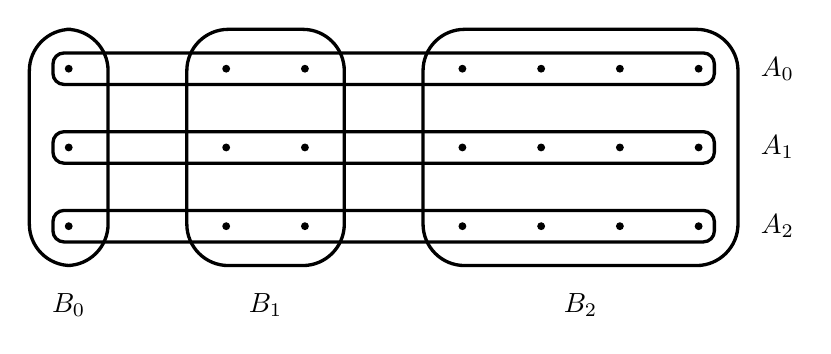
\begin{tikzpicture}
            \fill (0,0) circle (0.05);
            \fill (0,1) circle (0.05);
            \fill (0,2) circle (0.05);

            \fill (2,0) circle (0.05);
            \fill (2,1) circle (0.05);
            \fill (2,2) circle (0.05);
            \fill (3,0) circle (0.05);
            \fill (3,1) circle (0.05);
            \fill (3,2) circle (0.05);
            
            \fill (5,0) circle (0.05);
            \fill (5,1) circle (0.05);
            \fill (5,2) circle (0.05);
            \fill (6,0) circle (0.05);
            \fill (6,1) circle (0.05);
            \fill (6,2) circle (0.05);
            \fill (7,0) circle (0.05);
            \fill (7,1) circle (0.05);
            \fill (7,2) circle (0.05);
            \fill (8,0) circle (0.05);
            \fill (8,1) circle (0.05);
            \fill (8,2) circle (0.05);
            
            \draw[very thick, rounded corners=15pt]
              (-0.5,-0.5) rectangle ++(1,3);
            \draw[very thick, rounded corners=15pt]
              (1.5,-0.5) rectangle ++(2,3);
            \draw[very thick, rounded corners=15pt]
              (4.5,-0.5) rectangle ++(4,3);
              
            \draw[very thick, rounded corners=4pt]
              (-0.2,-0.2) rectangle ++(8.4,0.4);
            \draw[very thick, rounded corners=4pt]
              (-0.2,0.8) rectangle ++(8.4,0.4);
            \draw[very thick, rounded corners=4pt]
              (-0.2,1.8) rectangle ++(8.4,0.4);
              
            \node[] at (0,-1) {$B_0$};
            \node[] at (2.5,-1) {$B_1$};
            \node[] at (6.5,-1) {$B_2$};
            \node[] at (9,0) {$A_2$};
            \node[] at (9,1) {$A_1$};
            \node[] at (9,2) {$A_0$};
        \end{tikzpicture}
    \end{figure}
    Notice that $|A_i|=2^d-1$ for any $i$ and $|B_j|=k\cdot 2^j$ for $0\leq j<d$. Let's call this set cover $C_{d,k}=\{A_0, \ldots, A_{k-1}, B_0, \ldots, B_{d-1}\}$. If we fix some $k\geq 2$ (e.g. $k=3$ as the problem asks), we claim that running the greedy algorithm on $C_{d,k}$ returns a $\Omega(\log n)$ cover for all $d>0$.
    
    Fix some $k\geq 0$. Clearly $\{A_0,\ldots,A_{k-1}\}$ is the minimum set cover of $C_{d,k}$ for a sufficiently large $d$. In particular, it has constant size $k$. Note that $B_{d-1}$ is the maximal set in $C_{d,k}$, so the greedy set cover algorithm would add it to the generated set cover. The intersection of the remaining elements with the set cover is now equivalent to $C_{d-1,k}$. Again, the maximal set here is $B_{d-2}$. This proceeds inductively, generating the set cover $\{B_0,\ldots,B_{d-1}\}$ which of course has size $d$. Note that $\log n=\log (k(2^d-1))=\log k+\log(2^d-1) \geq d$ for $d$ large enough, so the size of the set is $\Omega(\log n)$.  
\end{solution}

\pagebreak
\begin{problem}
    ``Hey Upper East Siders, Gossip Girl here.'' You are secretly Gossip Girl, an anonymous gossip blogger who keeps track of friendships at Constance Billard High School. You publish an up-to-date map of the friendships at Constance on your website. You maintain this map by a stream of tips from anonymous followers of the form ``A is now friends with B." 

    \begin{enumerate}[(a)]
        \item {\bf (5 points)} You call some groups of people a ``squad'': each person is in the same squad as all their friends, and every member of a squad has some chain of friendships to every other member. Give an algorithm that takes in a stream of (a) tips and (b) requests for a specified person's squad name. You should answer requests that come in between tips consistently---if you make up the name ``The Billard billiards players'' for Dan's squad, and you're asked for Serena's squad's name before any new tips come in, you should report that it's ``The Billard billiards players''.
        \item {\bf (10 points)} A ``circular squad'' is defined to be a squad such that there is some pair of friends within the group that have both a friendship and a chain of friendships of length more than 1. Modify your algorithm from the previous part so that you report names that contain the word ``circle'' for all circular squads (and not for any other squads).
        \item {\bf (15 points)} Chatter Charlie, a rival gossip blogger, also begins to publish friendship maps informed by a stream of anonymous tips. Some tips are sent to just you, some just to him, and some to both of you. After you're both done taking tips for the year, it turns out that the whole school is a squad, and both you and Charlie know it. Give an algorithm to find the smallest subset of the tips that would've sufficed to convince both you and Charlie that the whole school was a squad.
    \end{enumerate}
\end{problem}

\begin{solution}
    \textbf{(a)} We store squads by first making a dynamically sized list of squad data structures, and an array indexed by students (we can associate each student to some $0,\ldots,n-1$) containing points to a squad object. Thus it's constant time to see what squad a student belongs to. The squad data structure contains an undirected adjacency list graph of all of the friendships which are in this squad, as well as a name. It's clear that any request to fetch the squad name of a given student will be constant, since it just involves getting the pointer to the squad object
    
    Every time we receive a tip of the form ``A is now friends with B'', we do the following:
    \begin{itemize}
        \item If neither A nor B are in a squad, create a new squad object named something random, and add students A and B to it. (This involves adding the A-B edge to the squad graph and setting pointers in the array of students)
        \item If one of A and B are in a squad and the other isn't, (assume without loss of generality that A is in a squad), we set the pointer for B to point for A's squad, and add the A-B edge to the squad graph.
        \item If both A and B are in the same squad, simply add the edge to the squad graph.
        \item If A and B are in different squads, we pick one of the squads (for example the larger one, say A) and merge the two groups together along the A-B edge. This involves overwriting all of the pointers in B's squad to point to A's squad, and merging the adjacency list graphs along the A-B edge (constant time complexity because of the adjacency list representation). We also need some procedure to combine the names of the squads, this can be chosen arbitrarily for instance ``Dan's Squad'' + ``Alice's Squad'' becomes ``Dan and Alice's Squad'' or something similar. 
    \end{itemize} 

    This is essentially a union find algorithm so it takes $O(n\log n)$ to process $n$ requests.

    \textbf{(b)} Let's add a boolean to the squad object which represents whether or not the squad is circular. By default it is set to false. Every time we add a new friendship, we then perform the following check in one of the options from the algorithm in (a):
    \begin{itemize}
        \item If A and B are both in the same squad (and there does not already exist an edge between them in the squad graph), set the squad as circular.
        \item If A and B are in different squads and we merge their squads, set the circularity of the full squad to be true if one of the squads is circular.
    \end{itemize}
    This clearly works, because a graph can't become acyclic by adding edges so we never set circular to false. Similarly, if we add an edge A-B to a connected graph which already contains A and B, we necessarily produce a cycle because since the graph is connected, there must already be a path from A-B. So including this new edge will produce a cycle of length greater than one. Lastly, we update the name generation method, so whenever the circularity of a squad is set true, we update the name by adding ``circle''. This doesn't add any time complexity to the algorithm.

    \textbf{(c)} Say you have graph represented by the edge set $E_1$ and Charlie has graph represented by the edge set $E_1$. These are stored in an adjacency list representation, maybe with some extra information to allow for easier iterating through the list of edges. Let $T$ be the final disjoint set of tips, represented by the same data structure we used to represent the set of squads. We'll create another disjoint set $T'$ to use as scratch space.

    We start by adding all of the edges which $E_1$ and $E_2$ have in common to $T'$. This can be done in $O(|E_1|)$ time. Then iterate through the edges in $T'$ and only add them to $T$ if there isn't already a node connecting the endpoints of the node we're adding. After this process completes, $T$ will contain the largest size acyclic subgraph of $E_1\cap E_2$. Next, we iterate over every student in the school. If $T$ doesn't contain the student this means that there is no edge in $E_1\cap E_2$ which connects the student to the set we're building, so add an edge from both $E_1$ and $E_2$ which connects the student to the set. After this process is complete, $T$ is connected, and both $T\cap E_1$ and $T\cap E_2$ are connected. This solution will indeed return the minimum set of tips. Suppose $T'$ were the minimum set of tips. Then $T'\cap (E_1\cap E_2)$ should be the minimum set of tips needed to connect $E_1\cap E_2$. However by our construction, $T\cap (E_1\cap E_2)$ has this exact property. Next, adding all of the other edges must be done in the way we do it, because since the students are not in $E_1\cap E_2$, they must have two distinct tips from $E_1$ and $E_2$ connecting them to the graph. Thus $|T'|=|T|$.
    
\end{solution}

\pagebreak
\begin{problem}
    On July 21st, 2019, our favorite TF, Tarun, participated in a 6-hour long Pokemon Go marathon.  Unfortunately, Tarun's backpack has limited carrying capacity. He has $M$ extra mudkips that he would like to give to his friends\ldots for a price. His trainer friends, including $t_0 = \text{Eric}$ and $t_1 = \text{Phyllis}$, are indicated by $T = \{t_0, \ldots, t_{|T|-1}\}.$ Each trainer $t_i$ would pay Tarun some positive integer $p_i$ dollars for some positive integer $m_i$ mudkips. The offers are all-or-nothing: each trainer $t_i$ will walk away with either $0$ or $m_i$ mudkips. Let a ``profile'' be a set of values of $M$, $|T|$, $p_i$, and $m_i$ as above. You can assume that for at least one $i$, $m_i \le M$. Consider the following two algorithms: 

    \begin{itemize}
        \item The ``value-per-mudkip'' greedy algorithm where Tarun selects, among the trainers whom he has enough mudkips to satisfy, the person offering the highest value per mudkip, sells them their requested mudkips, and repeats.
        \item The ``lazy'' greedy algorithm where Tarun decides that dividing is too difficult and selects, among the trainers whom he has enough mudkips to satisfy, the person offering the highest total price, sells them their requested mudkips, and repeats.
    \end{itemize}

    \hr

    \begin{enumerate}[(a)]
        \item {\bf (5 points)} Consider the profile where $$M=10, |T|=3, (m_0, m_1, m_2)=(10, 5, 1), (p_0, p_1, p_2) = \{8, 5, 1\}.$$ What does the ``value-per-mudkip'' greedy algorithm return? What does the ``lazy'' greedy algorithm return? What is the optimal allocation?
        \item {\bf (5 points)} Let the optimal allocation result in profit $P_\mathrm{opt}.$ Let the ``value-per-mudkip'' greedy algorithm result in profit $P_\mathrm{vpm}.$ Prove the smallest real number upper bound you can on $\dfrac{P_\mathrm{opt}}{P_\mathrm{vpm}}$, or prove that no such real number upper bound exists.
        \item {\bf (5 points)} The ``value-per-mudkip'' algorithm skips the next highest VPM trainer when they want more mudkips than Tarun has left. Suppose Tarun cheats a bit and sells to this highest trainer at full price even though he cannot allocate them all the mudkips they request---possibly even 0 mudkips. (Then Tarun flees town.) That is, Tarun sells to the first $k$ highest VPM trainers until he has either allocated more than $M$ mudkips or sold to all trainers. Prove the smallest real number upper bound you can on the ratio of $P_\mathrm{opt}$ to the profit from this ``illegitimate" auction, or prove that no such real number upper bound exists.
        \item {\bf (15 points)} Give a new algorithm such that $\dfrac{P_\mathrm{opt}}{P_\mathrm{new}}$ is always at most 2.
        % (\textbf{Hint:} Sorting by VPM, which trainers does the ``value-per-mudkip" greedy algorithm select? How does the value of the trainer Tarun cheats relate to the ``lazy" greedy algorithm?)
        \item {\bf (10 points)} Using your new algorithm from the previous part, show that for every $\epsilon > 0$, there exists some profile such that $\dfrac{P_{\mathrm{opt}}} {P_{\mathrm{new}}} \geq 2 - \epsilon$. This proves that your bound from the previous part is tight---you cannot find a better upper bound.
    \end{enumerate}
\end{problem}

\pagebreak
\begin{solution}
    \textbf{(a)} The VPM algorithm notes that the maximal value per mudkip trainers are $t_1$ and $t_2$, however $t_1$ sells more mudkips, so Tarun sells 5 mudkips for 5. Next, he sells 1 mudkip for 1, and he now only has 4 mudkips left and the only offer requires 10, so he's done with profit 6. The lazy greedy algorithm sells all ten mudkips for 8 to $t_0$. The optimal allocation is given by the lazy greedy algorithm in this case, with a profit of 8.
    
    \textbf{(b)} No upper bound exists. This is because for any $M>3$, we have the profile $|T|=2$, $(m_0, m_1)=(1, |M|-2),$ and $(p_0,p_1)=(1,|M|-3)$. The greedy algorithm will always return a profit of 1 and terminate, however the optimal allocation is $|M|-3$ dollars. So the ratio $\frac{P_{\mathrm{opt}}}{P_{\mathrm{vpm}}}=|M|-3$ which is unbounded.
    
    \textbf{(c)} We claim that $\frac{P_{\mathrm{opt}}}{P_{\mathrm{ill}}}\leq 1$. Clearly this bound is reached by the profile $|T|=1, m_0=|M|, p_0=1$, since both algorithms return the same profit of 1. To show that it's less than or equal to $1$, suppose we were give some arbitrary profile. There are two cases.
    \begin{itemize}
        \item If the illegitimate algorithm terminated because it sold to all the trainers, then the optimal set of trades is just to sell all of the mudkips so the ratio is equal to one.
        \item If the illegitimate algorithm terminated because it ran out of mudkips during the last trade, we claim this produces a trade equal to or better than optimal. This is because we selected the trainers with the best dollar per mudkip ratio, and we sold all of the mudkips, so any other sequence of legitimate trades which involves a trade not in our list would use a trainer whose dollar per mudkip ratio is lower, contradicting the assumption that the trade is optimal.
    \end{itemize}

    \textbf{(d)} Our algorithm is as follows. First, run the greedy VPM algorithm. If the greedy algorithm returns the entire set of trades, we are done. Otherwise, select the next best dollar per mudkip trade offer. If doing just that trade offer and no other yields more profit than the VPM list, do just that trade offer. Otherwise, do the VPM trades.

    Let's prove that the ratio for this algorithm is bounded by $2$. First of all, it's clear that $P_{\mathrm{new}} \leq P_{\mathrm{opt}}$. Let $V_1$ be the profit returned by VPM and let $V_2$ be the profit of the next most valuable trade as in the algorithm description. Note that $P_{\mathrm{ill}}=V_1+V_2$ so by (c), $V_1+V_2\geq P_{\mathrm{opt}}$. Since $P_{\mathrm{new}}=\max(V_1, V_2)$, we can combine the inequalities into 
    \[
        P_{\mathrm{opt}}\leq V_1+V_2\leq 2\max(V_1,V_2)=2P_{\mathrm{new}}\implies \frac{P_{\mathrm{opt}}}{P_{\mathrm{new}}}\leq 2 
    .\]   

    \textbf{(e)} Fix some $\epsilon>0$. Let $N$ be the closest integer so that $1 /N\leq \epsilon$. Consider the profile given by $M=2N, |T|=3, (m_0, m_1, m_2)=(2N, N, N),$ and $(p_0, p_1, p_2)=(2N+1, N, N)$. Then the value per mudkip values are $(v_0, v_1, v_2)=(1+1 /2N, 1, 1)$. It's clear that the algorithm would return a profit of $P_{\mathrm{new}} = 2N+1$, since the highest valued per mudkip values are the first two trainers, but among those, the first one has more profit since they can't both be selected. However $P_{\mathrm{opt}}=2N$ by simply selecting the lowest two mudkip per trainer trades. Then
    \[
        \frac{P_{\mathrm{opt}}}{P_{\mathrm{new}}}=\frac{2}{1+1 /2N} \geq 2\left(1-\frac{1}{2N}\right) = 2-\frac{1}{N}\geq 2-\epsilon
    .\] 
    This completes the proof.
\end{solution}

\end{document}